%% Journal of Biomedical Informatics -- submission source (single file). Compile: pdflatex main_jbi_en; bibtex main_jbi_en; pdflatex x2.
%% Cross-references to the Supplementary Material are read from supl_jbi_en.aux (package xr-hyper).
\documentclass[final,1p,times]{elsarticle}

\usepackage[utf8]{inputenc}
\usepackage[english]{babel}
\hyphenation{ep-i-lep-sy ep-i-lep-tic}   %
\usepackage{amsmath,amssymb}
\usepackage{booktabs}
\usepackage{adjustbox}
\usepackage{array}
\usepackage{longtable}
\usepackage{caption}
\captionsetup[table]{position=above}   %
\captionsetup{labelsep=period}   %
\addto\captionsenglish{\renewcommand{\figurename}{Fig.}}   %
\usepackage{url}
\makeatletter\g@addto@macro\UrlBreaks{\do\-\do\.}\makeatother\Urlmuskip=0mu plus 2mu
\usepackage{enumitem}
\usepackage{tikz}
\usetikzlibrary{arrows.meta,positioning,shapes.geometric}
\usepackage[hidelinks]{hyperref}
\newcommand{\figref}[1]{Fig.~\ref{#1}}
\newcommand{\tabref}[1]{Table~\ref{#1}}
\renewcommand{\eqref}[1]{Eq.~(\ref{#1})}
\usepackage{lineno}\linenumbers   %
\newcommand*\patchAmsMathEnvironmentForLineno[1]{\expandafter\let\csname old#1\expandafter\endcsname\csname #1\endcsname
  \expandafter\let\csname oldend#1\expandafter\endcsname\csname end#1\endcsname
  \renewenvironment{#1}{\linenomath\csname old#1\endcsname}{\csname oldend#1\endcsname\endlinenomath}}
\newcommand*\patchBothAmsMathEnvironmentsForLineno[1]{\patchAmsMathEnvironmentForLineno{#1}\patchAmsMathEnvironmentForLineno{#1*}}
\AtBeginDocument{\patchBothAmsMathEnvironmentsForLineno{equation}\patchBothAmsMathEnvironmentsForLineno{align}\patchBothAmsMathEnvironmentsForLineno{gather}\patchBothAmsMathEnvironmentsForLineno{multline}}
\hypersetup{pdfsubject={Journal of Biomedical Informatics, research paper submission}, pdfkeywords={electroencephalography; data leakage; covariate adjustment; normative modeling; model validation; confounding; epilepsy}}
\usepackage{xr-hyper}\externaldocument{supl_jbi_en}   %
\biboptions{sort&compress}

\journal{Journal of Biomedical Informatics}


\begin{document}

\begin{frontmatter}

\title{Covariate-adjustment leakage in patient-level EEG classification: effects of fitting population, repeated measurements, and audit replication}

\author[a]{Miftah Furqaanul Haq}
\author[a]{Dwi Sunaryono\corref{cor1}}
\ead{dwi@its.ac.id}
\author[a]{Muhammad Hasan Basri}
\cortext[cor1]{Corresponding author: Dwi Sunaryono, Department of Informatics, Institut Teknologi Sepuluh Nopember (ITS), Surabaya 60117, East Java, Indonesia.}

\affiliation[a]{organization={Department of Informatics, Institut Teknologi Sepuluh Nopember (ITS)},
            city={Surabaya 60117},
            state={East Java},
            country={Indonesia}}

\begin{abstract}
\textbf{Objective:} Regressing covariates such as age or recording era out of tabular clinical features is known to create spurious discrimination. The study extends the finding to repeated electroencephalography (EEG) measurements and control-fitted references and quantifies audit error frequencies.
\textbf{Methods:} The audit is a feature-shuffle test with and without adjustment on identical partitions, judged by two decision rules. Shuffling removes the EEG--label link but keeps the label--covariate association, so any discrimination gained stems from the adjustment. Simulations with known truth and semi-synthetic data (recorded EEG features, labels from covariates alone) from 200 patients of the Temple University Hospital EEG Epilepsy Corpus (TUEP) and an independent cohort of 299 subjects supplied the measurements. Analyses were exploratory; replication and reference experiments were preplanned.
\textbf{Results:} At the observed association, adjusting raw features created about 11 percentage points (pp) of area under the receiver operating characteristic curve (AUC) for nonlinear classifiers in both cohorts. Window-level logistic regression gained 6.6 pp in TUEP (2.8 pp with a matched training configuration), whereas patient-level logistic regression gained at most 1.1 pp in either cohort. With strict nesting, an adjustment fitted only on training controls leaked into this classifier (+4.3 pp, 95\% confidence interval 3.8 to 4.8), more than a random reference of equal size (+1.7 pp) in this cohort composition. In simulation, the control-reference leak persisted with 1,000 controls. Frozen rules raised 0 false alarms in 48 independent leakage-free simulation audits and detected all 48 leaking ones, whereas semi-synthetic data without a label--covariate association gave false alarms in up to 14.6\% of 20-replicate draws.
\textbf{Conclusion:} Whether adjustment created discrimination depended on its fitting population and training configuration, not on the classifier alone. Reporting archive performance with a feature-shuffle test with and without adjustment, a pilot-planned replicate number, and an acquisition-metadata baseline separates adjustment artifacts from disease information.
\end{abstract}

\begin{keyword}
electroencephalography \sep data leakage \sep covariate adjustment \sep normative modeling \sep model validation \sep confounding \sep epilepsy
\end{keyword}%

\end{frontmatter}

\section{Introduction}\label{sec:intro}

Machine learning on routine electroencephalography (EEG) has been proposed to support the diagnosis of epilepsy, but its markers remain outside clinical practice. In a systematic review, only 6 of 37 studies used at least 100 subjects \cite{lemoine2024}. Large clinical archives offer larger samples, but recordings made for clinical care differ between patient groups in ways unrelated to disease. A classifier can learn those differences instead of the disease \cite{ongly2024}. In the public Temple University Hospital (TUH) EEG Epilepsy Corpus (TUEP) \cite{obeid2016,veloso2017}, patients with epilepsy are younger and were recorded more often in particular eras and on particular devices (Section~\ref{sec:populasi}).

A common response is covariate adjustment, which regresses age, sex, or recording era out of the features, as in normative modeling, age-dependent quantitative EEG Z-scores, or ComBat harmonization \cite{marquand2016,rutherford2022,li2022harmnqeeg,jaramillojimenez2024}. Because adjustment is itself a fitted model, it can create the discrimination it is meant to remove \cite{hamdan2023}. The effect was shown for tabular data with one row per subject and an adjustment fitted on all subjects, two conditions from which clinical EEG pipelines depart.

Whether the leak appears and whether an audit detects it depend on three issues. The first two are these departures: classifiers are often fitted on windows, whereas adjustment is fitted on patients, and normative references are fitted on controls rather than on all training patients. In addition, audits have rested on few shuffles, although a single null area under the receiver operating characteristic curve (AUC) with 100 patients per class has a standard deviation (SD) of about 4 percentage points (pp, Section~\ref{sec:sensitivitas}). How much the three issues change the leak and the audit decisions has not been measured (Section~\ref{sec:related}), so archive performance figures after adjustment can mix disease information with adjustment artifacts.

The present study audits adjustment-induced discrimination at the patient level in repeated EEG measurements and shows how fitting population, fitting unit, and audit replication affect its conclusions. Established components make up the audit, namely a feature-shuffle test run with and without adjustment on identical partitions, two explicit decision rules, and a rule for the number of shuffles. Simulations with known truth and semi-synthetic data (plasmode, with recorded EEG features and labels from covariates alone) in two cohorts supply the measurements, and a fusion pipeline planned for TUEP is the clinical test case. The contributions address the three issues in turn:
\begin{itemize}[leftmargin=*,itemsep=0pt,topsep=2pt]
\item (i) Leak size and fitting unit. Adjusting raw EEG features without label information added about 11 pp of discrimination to nonlinear classifiers in two cohorts. Window-level logistic regression gained 6.6 pp in TUEP (2.8 pp with a matched training configuration), and patient-level logistic regression at most 1.1 pp.
\item (ii) Reference sample. An adjustment fitted only on training controls leaked into a linear patient-level classifier (+4.3 pp with strict nesting), more than a random reference of equal size (+1.7 pp) in this cohort composition. In simulation, the leak persisted with 1,000 reference controls.
\item (iii) Decision rules. On new simulation runs, the frozen rules raised 0 false alarms in 48 leakage-free audits and detected all 48 leaking ones, whereas null plasmode data gave false alarms in up to 14.6\% of draws of 20. A rule based on the mean and SD of pilot shuffles sets the number of shuffles when the pilot mean stays well below the margin (Section~\ref{sec:sensitivitas}).
\end{itemize}
The remaining sections review related work, describe the audit, report the measurements, and discuss the findings (Sections~\ref{sec:related}--\ref{sec:conclusion}), and \tabref{tab:signifikansi} states the significance.

\begin{table}[t]
\caption{Statement of Significance.}\label{tab:signifikansi}
\centering\small
\begin{tabular}{p{0.27\textwidth}p{0.66\textwidth}}
\toprule
Problem or Issue & Covariate adjustment of clinical EEG features can create spurious discrimination, so archive performance figures may reflect the adjustment instead of the disease. \\
What is Already Known & Regressing confounders out of tabular features can leak the label into nonlinear classifiers, and shuffling features before removal can reveal it. \\
What this Paper Adds & A patient-level audit showing that adjustment-created discrimination differed by fitting population (controls), fitting unit (windows), and audit replication, with rule error frequencies checked on independent simulation runs. \\
Who would benefit from the new knowledge in this paper & Researchers who build or evaluate clinical EEG and other patient-clustered models, and managers of clinical data archives. \\
\bottomrule
\end{tabular}
\end{table}%
\section{Related work}\label{sec:related}

Splitting by patient is the first safeguard against shortcuts in clinical EEG. Accuracies above 95\% have been reported on TUEP under a random 67/33 split \cite{rohira2023} and under segment-wise five-fold cross-validation \cite{tang2024}, and such figures mislead when segments of one patient fall on both sides of the split. In EEG of patients with Alzheimer's disease, an accuracy of 99.8\% under a segment-wise split fell to 53.0\% under a subject-wise split \cite{brookshire2024}, and pathology classification showed a similar gap \cite{delpup2025}. A patient-wise split removes this inflation, whereas acquisition shortcuts remain and escape internal cross-validation \cite{ongly2024}.

Covariate adjustment can err in two directions, and the first is the removal of biological signal. Harmonization may remove biological variance confounded with site \cite{bayer2022frontneurol}, and covariate regression fitted on training and test data together lowered the performance of connectome-based models \cite{rosenblatt2024}. In the second direction, Hamdan et al. showed on tabular data that removing confounders by per-feature regression, even inside the folds, adds spurious signal by moving confounder information into non-normal residuals that nonlinear classifiers exploit \cite{hamdan2023}. The removal in that study was fitted on all training subjects with one row per subject, and linear models showed no evidence of leakage, although leakage was not excluded. Normative models, in contrast, are trained on controls only \cite{rutherford2022,bayer2022neuroimage,kia2022}. Within one clinical archive, controls are the patients without the disease, so the fitting patients are selected by the label.

Tests for leakage build on the proposal of Hamdan et al. to shuffle the features before removal and to compare performance with and without removal. The main analyses of that study used a single shuffle, and a 1,000-iteration permutation test appeared only in a supplementary analysis. Hamdan et al. were not aware of a procedure that rules out this leakage \cite{hamdan2023}. The partial confounder test controls its type I error but asks whether predictions depend on a confounder given the label \cite{spisak2022}, not whether an adjustment creates discrimination. What was known and what this study adds are listed in \tabref{tab:diketahui}.

\begin{table}[t]
\caption{What was known and what this study adds.}\label{tab:diketahui}
\centering\scriptsize
\setlength{\tabcolsep}{3pt}
\begin{tabular}{p{0.30\textwidth}p{0.42\textwidth}p{0.20\textwidth}}
\toprule
Known before & Added by this study & Evidence \\
\midrule
Regression adjustment leaks into nonlinear models on tabular data with one row per subject \cite{hamdan2023} & (i) Leak size on recorded EEG features in two cohorts by classifier, fitting level (windows or patients), and transformation & Fig.~\ref{fig:peta}, Fig.~\ref{fig:plasmode} \\
Normative references are fitted on controls \cite{rutherford2022,kia2022}, and linear models showed no evidence of leakage when removal used all subjects \cite{hamdan2023} & (ii) A control-referenced adjustment leaks into a linear classifier, more than a random reference of equal size in this cohort composition. In simulation, the leak grows with the label--covariate association and shrinks by 2.7 pp from 80 to 1,000 controls & \tabref{tab:kebocoran_badan}, Fig.~\ref{fig:referensi} \\
Shuffling features reveals the leak, but a decision rule and an error rate were lacking \cite{hamdan2023} & (iii) Two rules with false-alarm and detection frequencies from replicate pools, checked on independent simulation runs, and a replicate-number rule & \tabref{tab:oc} \\
\bottomrule
\end{tabular}

\vspace{2pt}
\begin{minipage}{\textwidth}\footnotesize
Numerals (i)--(iii) match the contributions in Section~\ref{sec:intro}, and the full matrix is Table~\ref{tab:matriks}.
\end{minipage}
\end{table}%
\section{Methods}\label{sec:methods}

Internal codes appear only in tables, figures, and the Supplementary Material, whose sections are cited as S1--S4 (S1.6).

\subsection{Data and ethics}\label{sec:desain}

The study used TUEP v2.0.1 from the Neural Engineering Data Consortium (NEDC) and represented each of its 200 patients (100 with and 100 without epilepsy) by the first session in the corpus (2003--2013, 19 scalp electrodes) \cite{veloso2017,obeid2016}. Patients without epilepsy (``controls'') are clinical controls who also underwent EEG, not healthy volunteers. Labels came from TUEP curation based on the session report, clinical history, medication, and EEG features \cite{veloso2017}. Age, sex (female or male as recorded in the corpus; gender was not available), and recording era ($\leq$2009, 2010, 2011, 2012, 2013) served as covariates. An independent Emotiv cohort (Zenodo 1252141, consumer-grade resting-state EEG \cite{vanhees2018}) repeated the plasmode with 299 of its 313 subjects, those keeping at least five 10-s windows below label-free amplitude and head-motion thresholds (S2.11, S2.19).

The two datasets are public and de-identified, and NEDC distributes TUEP under its data use terms. Collection of the TUH corpus was approved by the Temple University institutional review board \cite{obeid2016}. As a secondary analysis of public, de-identified data, the study was exempt from approval by the authors' institutional ethics committee. The analysis used the released records without patient contact, re-identification, or record linkage (S1.7).

\subsection{Preprocessing, features, and adjustment}\label{sec:praproses}

Signals were average-referenced, resampled to 200 Hz, and filtered at 0.5--45 Hz. Windows of 10 s exceeding 800~$\mu$V peak to peak were rejected without using labels (2.3\% of windows) \cite{gemein2020,kiessner2024,poziomska2026}. The spectral view used log relative power in five bands and log total power on 19 channels (114 features, Welch's method), summarized per patient as the median over windows. L2-penalized logistic regression with balanced class weights classified the patient medians, with the regularization strength chosen from nine values by inner 5-fold cross-validation. A planned fusion pipeline averaged the probabilities of this view, a spatial view, and a temporal view (S3.5).

\label{sec:model}Adjustment regressed the feature vector $\mathbf{x}_i$ of each patient $i$ on the design vector $\mathbf{d}_i$ (intercept, age, sex, and era indicators) by ordinary least squares over a fitting set $\mathcal{P}_{\mathrm{tr}}$ of training patients (\eqref{eq:norm}). The residuals were divided element-wise ($\oslash$) by the residual standard deviations $\hat{\boldsymbol{\sigma}}$ of the fitting set.
\begin{equation}\label{eq:norm}
\hat{\mathbf{B}}=\arg\min_{\mathbf{B}}\sum_{j\in\mathcal{P}_{\mathrm{tr}}}\left\|\mathbf{x}_j-\mathbf{B}^{\top}\mathbf{d}_j\right\|^{2},\qquad
\mathbf{z}_i=\left(\mathbf{x}_i-\hat{\mathbf{B}}^{\top}\mathbf{d}_i\right)\oslash\hat{\boldsymbol{\sigma}}
\end{equation}
The planned pipeline used only the training controls as $\mathcal{P}_{\mathrm{tr}}$ (control-referenced adjustment), as normative references do \cite{rutherford2022,rutherford2023}, whereas the all-patient adjustment used all training patients. Variants used half of the training controls, cross-fitting, a design without era, or a random reference (Section~\ref{sec:metode_referensi}), and recording device entered only the acquisition-metadata baseline.

\subsection{The audit procedure}\label{sec:sensitivitas}

Steps of the audit and its training--test boundaries are shown in \figref{fig:alur}. The feature-shuffle test followed Hamdan et al. \cite{hamdan2023}: EEG features were permuted between patients before the split, each patient keeping its label and covariates, and the complete pipeline was run with and without adjustment on identical folds (S1.1). Under this between-patient shuffle, EEG is independent of the label and the covariates, while the label--covariate association is preserved. Any AUC above chance after adjustment therefore indicates adjustment-induced leakage. A within-era shuffle keeps the associations of EEG with era and of era with the label, so its AUC lacks a universal chance level of 50. The within-era shuffle serves only as a conditional sensitivity test, reported as the AUCs of both pipelines and the paired difference of the two, with a 95\% confidence interval (CI) and without a decision. Age and sex were removed from the classifier inputs in all null experiments. ``Leak'' denotes the measured excess discrimination in pp, and ``leakage'' the phenomenon and the decision label.

\renewcommand{\topfraction}{0.92}\renewcommand{\textfraction}{0.05}
\begin{figure}[t]
\centering
\begin{adjustbox}{max width=\textwidth}
\definecolor{aksen}{RGB}{212,171,106}
\begin{tikzpicture}[x=1cm,y=1cm,font=\sffamily\scriptsize,line width=0.5pt,
  panel/.style={font=\sffamily\scriptsize\bfseries,anchor=north west,inner sep=0pt},
  bx/.style={draw=black,inner sep=2.6pt,align=left,anchor=north west},
  dat/.style={bx,fill=black!8},
  prc/.style={bx,fill=white},
  adj/.style={bx,draw=aksen,line width=0.8pt,fill=aksen!7},
  frm/.style={draw=black,anchor=north west,inner sep=0pt},
  hd/.style={anchor=north west,align=left,inner sep=1.5pt},
  mk/.style={anchor=east,align=right,font=\sffamily\scriptsize\itshape,text=black!70,inner sep=1pt},
  tg/.style={anchor=north east,font=\sffamily\scriptsize\bfseries,inner sep=1.5pt},
  nt/.style={anchor=north west,align=left,font=\sffamily\scriptsize,text=black!70,inner sep=1pt},
  flow/.style={-{Stealth[length=1.6mm,width=1.2mm]},line width=0.6pt},
  frz/.style={-{Stealth[length=1.6mm,width=1.2mm]},line width=0.6pt,dashed},
  lbl/.style={font=\sffamily\scriptsize,inner sep=1pt},
  every node/.append style={execute at begin node={\hyphenpenalty=10000\exhyphenpenalty=10000}}]

\node[panel] at (0,0) {(a)\hspace{4pt}Data and label-free feature extraction, per recording};
\node[dat,text width=2.72cm,minimum height=2.3cm] (a1) at (0,-0.45) {\textbf{TUEP v2.0.1}\\200 patients (100 with, 100 without epilepsy), first session only, 19 channels};
\node[prc,text width=2.92cm,minimum height=2.3cm] (a2) at (3.45,-0.45) {\textbf{Preprocessing}\\average reference, 200~Hz, 0.5--45~Hz; clean 10~s windows (26,968)};
\node[prc,text width=4.62cm,minimum height=2.3cm] (a3) at (7.1,-0.45) {\textbf{Feature views}\\[1pt]\textbf{I2} spectral: 114 log band-power features, median per patient\\[1pt]\textbf{P3} spatial: $18\times18$ covariance, tangent space (855), PCA (50)\\[1pt]\textbf{NM} temporal: 4~s segments, Mamba};
\node[dat,text width=3.32cm,minimum height=2.3cm] (a4) at (12.45,-0.45) {\textbf{Per patient}\\features $\mathbf{x}_i$, covariates $\mathbf{d}_i$ (age, sex, era), label $y_i$};
\draw[flow] (a1.east) -- (a2.west);
\draw[flow] (a2.east) -- (a3.west);
\draw[flow] (a3.east) -- (a4.west);

\node[panel] at (0,-3.05) {(b)\hspace{4pt}Patient-level nested evaluation, one prediction per patient};
\node[prc,text width=15.77cm] (sp) at (0,-3.55) {\textbf{Patient-level split}: 10 repetitions $\times$ 5 stratified folds = 50 splits, identical for all models; all windows of a patient stay in one fold};
\draw[flow] (a4.south) -- (a4.south |- sp.north);
\draw[fill=black!15] (0,-4.02) rectangle (9.05,-4.42);
\foreach \xx in {2.2625,4.525,6.7875} \draw (\xx,-4.02) -- (\xx,-4.42);
\draw[fill=white] (9.75,-4.02) rectangle (15.95,-4.42);
\node[lbl,fill=black!15,inner sep=2pt] at (4.525,-4.22) {training folds (4 of 5)};
\node[lbl] at (12.85,-4.22) {test fold (1 of 5)};
\draw[flow] (4.525,-4.42) -- (4.525,-4.85); \node[lbl,anchor=west] at (4.6,-4.635) {160 patients};
\draw[flow] (12.85,-4.42) -- (12.85,-4.85); \node[lbl,anchor=west] at (12.925,-4.635) {40 patients};

\draw[line width=0.8pt,fill=black!4] (0,-4.85) rectangle (9.05,-9.5);
\node[hd,font=\sffamily\scriptsize\bfseries] at (0.08,-4.9) {Outer training fold: 160 patients};
\node[adj,text width=6.0cm,minimum height=0.85cm] (s1) at (0.35,-5.3) {\textbf{1\enspace Covariate adjustment} (Eq.~(1)), fitted on all training patients: V4 (I2, NM) or V5 (P3); null-test variant V0, training controls selected by label};
\node[prc,text width=6.0cm,minimum height=0.5cm] (s2) at (0.35,-6.45) {\textbf{2\enspace Scaler, reference covariance, PCA}, same patients};
\node[prc,text width=6.0cm,minimum height=0.85cm] (s3) at (0.35,-7.25) {\textbf{3\enspace Inner selection}: regularization by 5-fold CV (I2, P3); NM: 80/20 split for configuration and early stopping};
\node[prc,text width=6.0cm,minimum height=0.5cm] (s4) at (0.35,-8.4) {\textbf{4\enspace Final classifier} fitted on the 160 patients};
\draw[flow] (s1.south) -- (s2.north);
\draw[flow] (s2.south) -- (s3.north);
\draw[flow] (s3.south) -- (s4.north);
\node[mk] at (8.95,-5.725) {label-free}; \node[mk] at (8.95,-6.7) {label-free};
\node[mk] at (8.95,-7.675) {uses labels}; \node[mk] at (8.95,-8.65) {uses labels};
\node[nt,text width=8.7cm] at (0.08,-9.05) {Strict-nesting sensitivity: steps 1--2 refitted in each inner split.};

\draw[line width=1.0pt,dash pattern=on 4pt off 2.5pt] (9.4,-4.02) -- (9.4,-9.75);
\node[font=\sffamily\scriptsize,rotate=90,fill=white,inner sep=1.5pt] at (9.4,-8.3) {training--test boundary};

\draw[line width=0.8pt,fill=white] (9.75,-4.85) rectangle (15.95,-9.5);
\node[hd,font=\sffamily\scriptsize\bfseries] at (9.83,-4.9) {Outer test fold: 40 patients};
\node[prc,text width=5.52cm,minimum height=0.85cm] (s5) at (10.05,-5.3) {\textbf{5\enspace Frozen transforms and classifier} from steps 1--4; no refitting};
\node[prc,text width=5.52cm,minimum height=0.5cm] (s6) at (10.05,-6.45) {\textbf{6\enspace One probability per patient} and view (I2, P3, NM)};
\node[prc,text width=5.52cm,minimum height=0.5cm] (f2) at (10.05,-7.25) {\textbf{F2}: mean of the three probabilities};
\node[prc,text width=5.52cm,minimum height=0.85cm] (auc) at (10.05,-8.05) {\textbf{Per-fold AUC} over 50 folds (clinical label); Nadeau--Bengio 95\% CI};
\draw[flow] (s5.south) -- (s6.north);
\draw[flow] (s6.south) -- (f2.north);
\draw[flow] (f2.south) -- (auc.north);
\node[nt,text width=5.9cm] at (9.83,-9.05) {Held out from fitting and selection.};
\draw[frz] (9.05,-5.725) -- (s5.west);

\node[panel] at (0,-10.0) {(c)\hspace{4pt}Audit layer: feature-shuffle test, run with and without adjustment};
\node[frm,minimum width=3.0cm,minimum height=3.3cm] (c1) at (0,-10.45) {};
\node[frm,minimum width=3.7cm,minimum height=3.3cm] (c2) at (3.45,-10.45) {};
\node[frm,minimum width=2.8cm,minimum height=3.3cm] (c3) at (7.6,-10.45) {};
\node[frm,minimum width=5.1cm,minimum height=3.3cm] (c4) at (10.85,-10.45) {};
\draw[flow] (c1.east) -- (c2.west);
\draw[flow] (c2.east) -- (c3.west);
\draw[flow] (c3.east) -- (c4.west);
\node[hd,text width=2.8cm] at (0.03,-10.5) {\textbf{Null data}\\[1pt]Patients keep label $y_i$ and covariates $\mathbf{d}_i$; EEG features $\mathbf{x}_i$ are permuted between patients (H1) or within era (H2a). Age and sex are excluded from classifier inputs.};
\node[tg,anchor=south east] at (3.0,-13.75) {(i)};
\node[hd,text width=3.5cm] at (3.48,-10.5) {\textbf{Pipeline, run twice}\\same permutation, folds, and classifier};
\node[adj,text width=3.3cm,minimum height=0.62cm] (cw) at (3.56,-11.55) {with adjustment\\(Eq.~(1)): AUC $A_r$};
\node[prc,text width=3.3cm,minimum height=0.62cm] (co) at (3.56,-12.5) {without adjustment:\\AUC $A_r^{0}$};
\node[tg,anchor=south east] at (7.15,-13.75) {(i), (ii)};
\draw[fill=white] (7.9,-10.75) rectangle (10.25,-13.2);
\draw[fill=white] (7.8,-10.85) rectangle (10.15,-13.3);
\draw[fill=white] (7.7,-10.95) rectangle (10.05,-13.4);
\node[hd,text width=2.2cm] at (7.73,-11.05) {\textbf{Replicates}\\$r=1,\dots,n$\\[3pt]$\Delta_r=A_r-A_r^{0}$\\[3pt]means $\bar{A}$ and $\bar{\Delta}$ with Monte Carlo SE (Eq.~(2))};
\node[hd,text width=4.9cm] at (10.88,-10.5) {\textbf{Decision per rule} (Eq.~(3))};
\fill[black!12] (11.1,-11.2) rectangle (12.5,-11.45);
\fill[aksen!30] (14.4,-11.2) rectangle (15.75,-11.45);
\draw (11.1,-11.2) rectangle (15.75,-11.45);
\foreach \xx/\lab in {12.5/\ell,13.45/u,14.4/\lambda} {\draw (\xx,-11.12) -- (\xx,-11.53); \node[lbl,anchor=south] at (\xx,-11.12) {$\lab$};}
\node[lbl,font=\sffamily\tiny] at (11.8,-11.65) {no evidence};
\node[lbl,font=\sffamily\tiny] at (13.45,-11.65) {uncertain};
\node[lbl,font=\sffamily\tiny] at (15.075,-11.65) {leakage};
\node[hd,text width=4.9cm] at (10.88,-11.85) {no evidence: $m\leq\ell$ and $m+1.645\,\mathrm{SE}\leq u$\\leakage: $m>\lambda$; uncertain otherwise\\[2pt]\begin{tabular}{@{}l@{\ }l@{}}absolute:&$m=\bar{A}$, $(\ell,u,\lambda)=(52.0,54.0,55)$\\paired:&$m=\bar{\Delta}$, $(1.0,3.0,3.0)$ pp\end{tabular}\\[2pt]combined: leakage if any rule declares it};
\node[tg,anchor=south east] at (15.95,-13.75) {(iii)};
\draw[line width=0.5pt] (0,-14.25) -- (15.95,-14.25);
\node[lbl,anchor=south west] at (0,-14.23) {Claims tested with this audit; tags (i)--(iii) in the boxes mark the stage each claim varies};
\node[lbl,anchor=south east] at (15.95,-14.23) {clinical-label checks: S3.5};
\node[prc,text width=4.92cm,minimum height=1.2cm] at (0,-14.45) {\textbf{(i) Leak size}: simulation with a known truth and plasmode on recorded EEG features of TUEP and Emotiv; classifier, fitting unit, and transformation varied};
\node[prc,text width=4.92cm,minimum height=1.2cm] at (5.42,-14.45) {\textbf{(ii) Reference sample}: $\mathcal{P}_{\mathrm{tr}}$ = training controls, all training patients, or equally many random training patients; reference size varied in simulation};
\node[prc,text width=4.92cm,minimum height=1.2cm] at (10.85,-14.45) {\textbf{(iii) Rule errors}: absolute (R1) and paired (R2) rules, alone and combined, on stored replicates and on new simulation runs; false alarms and detections};

\draw[flow] (6.9,-16.0) -- (7.7,-16.0); \node[lbl,anchor=west] at (7.8,-16.0) {data flow};
\draw[frz] (9.3,-16.0) -- (10.1,-16.0); \node[lbl,anchor=west] at (10.2,-16.0) {frozen parameters};
\node[adj,minimum width=0.6cm,minimum height=0.25cm,inner sep=0pt,anchor=west] at (12.55,-16.0) {}; \node[lbl,anchor=west] at (13.25,-16.0) {covariate adjustment};
\end{tikzpicture}
\end{adjustbox}
\caption{Audit workflow. (a) Label-free preprocessing per recording. (b) Steps 1--4 are fitted on the 160 training patients, and the 40 test patients receive the frozen transforms and classifier. Labels enter only in steps 3--4, except that the null-test variant V0 selects its reference patients by label in step 1. (c) The feature-shuffle test runs the pipeline with and without adjustment on the same permutation and folds, and two rules judge the replicate means. I2, P3, and NM, spectral, spatial, and temporal views; F2, fusion; V4 and V5, all-patient adjustments; H1 and H2a, shuffles; R1 and R2, rules. CV, cross-validation; PCA, principal component analysis; SE, standard error; AUC, area under the receiver operating characteristic curve; pp, percentage points; CI, confidence interval; TUEP, Temple University Hospital EEG Epilepsy Corpus.}\label{fig:alur}
\end{figure}%

Let $A_r$ and $A_r^{0}$ denote the AUCs (in percent) of shuffle replicate $r=1,\dots,n$ with and without adjustment on the same permutation and folds (per-fold or pooled, S1.3), let $\Delta_r=A_r-A_r^{0}$, and let $\hat{\sigma}_{\Delta}$ be the sample SD of the $\Delta_r$. The audit summarizes
\begin{equation}\label{eq:bocor}
\bar{A}=\frac{1}{n}\sum_{r=1}^{n}A_r,\qquad
\bar{\Delta}=\frac{1}{n}\sum_{r=1}^{n}\Delta_r,\qquad
\mathrm{SE}(\bar{\Delta})=\frac{\hat{\sigma}_{\Delta}}{\sqrt{n}},
\end{equation}
with the standard error $\mathrm{SE}(\bar{A})$ analogous, both measuring Monte Carlo error over replicates. Replicate means enter both rules, because a single null AUC with 100 patients per class has an SD of 4.1 pp (Mann--Whitney variance, S1.1). The absolute rule ($m=\bar{A}$) and the paired rule ($m=\bar{\Delta}$, between-patient shuffle only) share one form,
\begin{equation}\label{eq:aturan}
\text{decision}(m)=
\begin{cases}
\text{no evidence of leakage}, & m\leq\ell \text{ and } m+1.645\,\mathrm{SE}(m)\leq u,\\
\text{leakage}, & m>\lambda,\\
\text{uncertain}, & \text{otherwise},
\end{cases}
\end{equation}
with $(\ell,u,\lambda)=(52.0,54.0,55)$ for the absolute rule and $(1.0,3.0,3.0)$ pp for the paired rule, where $m+1.645\,\mathrm{SE}(m)$ is the one-sided 95\% upper bound. In the combined decision, a pipeline is leaking when any rule computed for it declares leakage, and it shows no evidence of leakage only when all such rules say so. The label ``no evidence'' means within the stated tolerance, not zero leakage. Margin-test conventions, as in equivalence testing, set these thresholds. Mean thresholds of 52 and 55 were fixed before the first audit, and the upper-bound condition was added after the first audits (S1.5). If paired null differences have mean $b$ and SD $\sigma_{\Delta}$, the false-alarm frequency of the paired rule with $\lambda=3$ pp under a normal model is
\begin{equation}\label{eq:n}
\Pr\left(\bar{\Delta}>\lambda\right)=1-\Phi\left(\frac{(\lambda-b)\sqrt{n}}{\sigma_{\Delta}}\right)<1\%\quad\text{if } n\geq\left(\frac{2.33\,\sigma_{\Delta}}{\lambda-b}\right)^{2},\ b<\lambda,
\end{equation}
where $\Phi$ is the standard normal distribution function. A pilot applies the same pipeline to a negative control without a label--covariate association. Under this model, the 1\% target holds for the paired rule only, whereas the combined decision has its own frequencies (Section~\ref{sec:oc}, worked example in S2.19). The planning rule was formulated after the decision frequencies had been measured. Bootstrap draws of $n$ replicates from stored pools (S2.17) and non-overlapping audits of 2,000 new simulation replicates in null (leakage-free), near-margin, and leaking cells (S2.18) supplied those frequencies, with Clopper--Pearson intervals for audit counts.

\subsection{Simulation and plasmode}\label{sec:metode_peta}

The simulation generated clustered data without a disease signal (base cell of 200 patients, 50 windows, and 50 features) from normal, lognormal, $t$, chi-squared, or contaminated distributions. Covariates resembled those of TUEP with a label--covariate association $s\in\{0,0.5,1\}$, and one factor varied at a time. The comparison crossed four transformations (raw, symlog, rank-normal, log), adjustment of windows or of patient means, and five classifiers on identical data and folds (S1.8). Logistic regression, random forest, XGBoost, a multilayer perceptron, and a bidirectional long short-term memory network (Bi-LSTM) formed the classifier set.

The plasmode, a semi-synthetic design, combined recorded EEG features with synthetic labels
\begin{equation}\label{eq:plasmode}
\tilde{y}_i=\mathbf{1}\left[\gamma\eta_i+\epsilon_i\geq\tau_{\gamma}\right],\qquad \epsilon_i\sim\mathrm{Logistic}(0,1),\qquad \gamma\in\{0,0.5,1\},
\end{equation}
where $\eta_i$ is the linear predictor of a logistic regression of the clinical label on age, sex, and era, and $\tau_{\gamma}$ is the $\lfloor N/2\rfloor$-th largest score. Setting $\gamma=1$ mimics the observed association, and the threshold labels 100 of the 200 TUEP patients as 1. Features were the spectral view, the window features of Rohira et al. \cite{rohira2023}, the per-second features of Tang et al. \cite{tang2024}, and temporal-view segments. The primary family (Holm) compared raw with rank-normal adjustment for the random forest, XGBoost, and the Tang Bi-LSTM, and a check required ``no evidence'' in at least 95\% of cells at $\gamma=0$. Raw tree pools were later extended from 20 or 30 to 120 replicates (S2.11). Follow-ups planned before computation repeated the plasmode on the 299 Emotiv subjects, with labels from that cohort's acquisition covariates. Further follow-ups fitted logistic regression to the raw window features of the trees (S2.12). Other follow-ups crossed training patients, window weights, and score aggregation (S2.16) and compared adjustment within each transformation (S2.15).

\subsection{Reference experiments}\label{sec:metode_referensi}

A simulation planned before computation (S2.13) tested the control-referenced adjustment against a known truth. Labels were balanced and TUEP covariate rows were resampled, while 114 normal features with the correlation of the spectral features were independent of label and covariates. The simulation crossed the number of training controls per fold (20, 40, 80, 200, or 1,000), the era design, and $s\in\{0,0.5,1\}$, with 100 replicates per cell. In the sparse design, about 6\% of controls fell into the earliest era, as in TUEP. The mirror design swapped the source rows of the classes, preserving the association but moving the sparse cell to the cases. Holm correction over three one-sided Welch tests covered the primary family, which compared 80 with 1,000 controls, the sparse with the mirror design, and $s=1$ with $s=0$. A second experiment (S2.14) repeated the null test on the same 100 permutations with a random reference of 80 training patients drawn regardless of label, with the paired difference from the control reference as its frozen contrast.

\subsection{Validation and statistics}\label{sec:validasi}

Null experiments on recorded features used 10 repetitions of five stratified patient-level folds (160 training, 40 test patients), and simulations and plasmode one new split per replicate. The windows of a patient stayed in one fold, and any step that estimates statistics across patients was fitted on the training patients of the fold \cite{varma2006,rosenblatt2024,delpup2025,brookshire2024}. Automated leakage checks passed on all 50 folds (S2.9). The per-fold AUC averages test-fold AUCs, and the pooled AUC uses the out-of-fold scores of a repetition (S1.3). Differences over replicates were tested with $t$-tests (one-sided where the plan fixed a direction) and Holm correction within each family \cite{holm1979}, conditional on the same patients \cite{bates2024}; the clinical-label comparison used the Nadeau--Bengio corrected $t$-test \cite{nadeau2003}. Label-free transforms and the adjustment reference were fitted on the whole outer training fold before the inner selection of the regularization strength. Refitting the transforms and the reference within each inner split changed the per-fold AUC of clinical-label models by at most 0.3 pp (S2.10) and lowered the control-reference leak (Section~\ref{sec:kebocoran}, S2.19).

Design choices were iterated over 53 rounds of analysis on the same patients and folds without a hidden test set. The plan of each round was written in a version-controlled or SHA-256-hashed document after earlier results were known, so all analyses are exploratory (S1.5). By contrast, the Emotiv replication, the reference experiments, and the follow-ups of rounds 55--61 were planned before computation. Hyperparameters are listed in Table~\ref{tab:hiper}, and reporting followed TRIPOD+AI \cite{collins2024tripod}.%
\section{Results}\label{sec:results}

AUCs are in percent (per-fold unless labeled pooled) and differences in pp; intervals over replicates on the same patients are Monte Carlo intervals.

\subsection{Cohort}\label{sec:populasi}

In TUEP, patients with epilepsy were younger (median age 52 against 59 years, Mann--Whitney $p = 0.002$) and were recorded in different eras and on different devices (chi-squared $p = 0.0013$ and $p = 0.0096$, Table~\ref{tab:kohort}). The earliest era held 25 patients with epilepsy and 6 controls.

\subsection{Size of the leak in simulation and on recorded EEG features}\label{sec:peta}

Because the TUEP label is associated with age and era, the first question was what adjusting for age and era creates without label information, with all adjustments in this subsection fitted on all training patients.

\begin{figure}[!htbp]
\centering
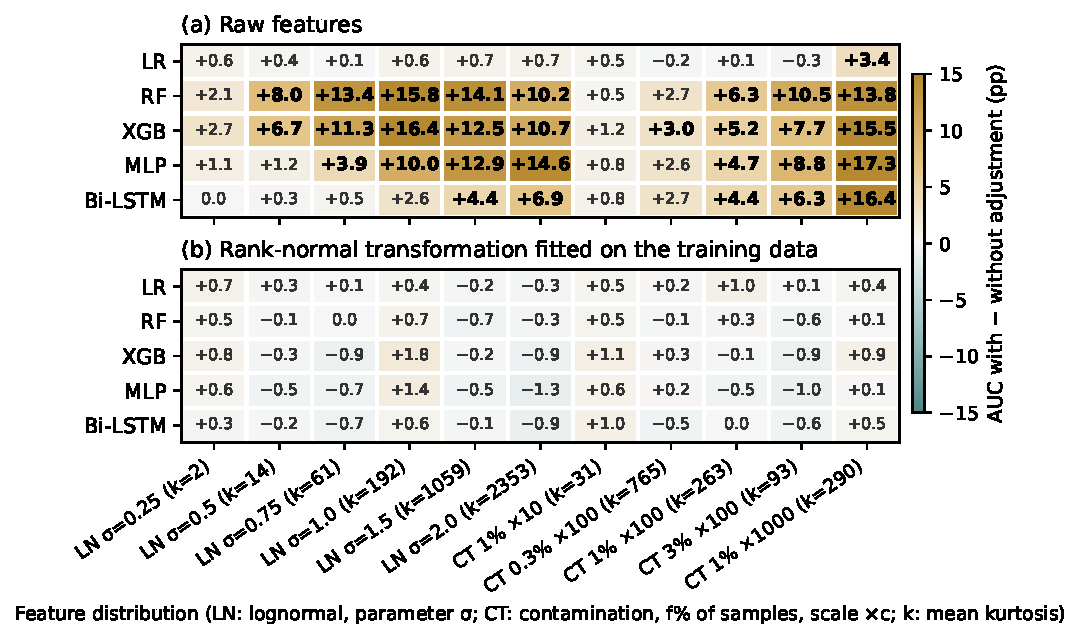
\includegraphics[width=\textwidth]{Fig2.pdf}
\caption{Leak created by adjusting patient means in simulation without a disease signal (200 patients, 50 windows, 50 features): paired difference in pooled AUC on (a) raw and (b) rank-normal features, labeled only above the 3-pp paired-rule threshold. AUC, area under the receiver operating characteristic curve, in percentage points (pp); LR, patient-level logistic regression; RF, random forest; XGB, XGBoost; MLP, multilayer perceptron.}\label{fig:peta}
\end{figure}

In simulation without a disease signal, adjustment of patient means raised the AUC of nonlinear classifiers when features were heavy-tailed (\figref{fig:peta}). Mean per-fold differences were +6.5 pp for raw features (60.0\% of cells ``leakage'') and +3.9 pp for symlog, whereas log and rank-normal stayed within 0.2 pp of zero. Patient-level logistic regression changed by at most +2.6 pp per fold across 134 cells. Higher intraclass correlation of the windows did not enlarge the leak of a window-level random forest (Holm-adjusted $p = 0.79$, S2.10). Recorded band-power features were heavy-tailed as well (median over features of the excess kurtosis across windows, 8,481 in TUEP and 75.9 in Emotiv, \tabref{tab:kurtosis}), as in the leaking simulation cells.

\begin{figure}[!htbp]
\centering
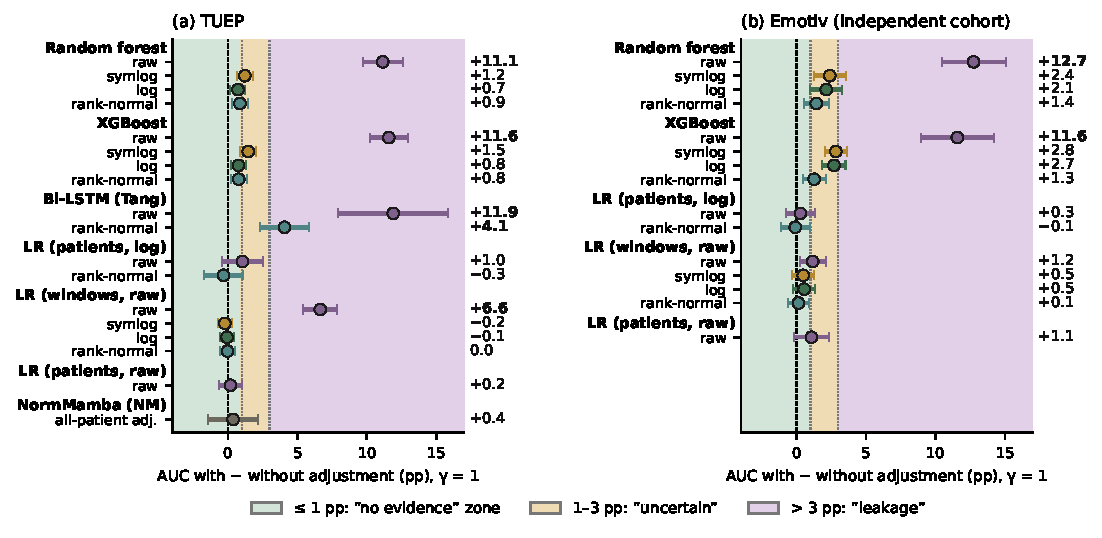
\includegraphics[width=\textwidth]{Fig3.pdf}
\caption{Leak created by covariate adjustment in the plasmode (between-patient shuffle, observed label--covariate association $\gamma=1$) in (a) TUEP and (b) Emotiv. Points are replicate means of the per-fold AUC difference between each pipeline with adjustment and the same pipeline and transformation without it, with Monte Carlo 95\% CIs. Shading, paired-rule mean thresholds; ``no evidence'' also requires the Monte Carlo upper bound of \eqref{eq:aturan} to stay at or below 3 pp. AUC, area under the receiver operating characteristic curve; pp, percentage points; CI, confidence interval; LR, logistic regression; Bi-LSTM, bidirectional long short-term memory network; TUEP, Temple University Hospital EEG Epilepsy Corpus.}\label{fig:plasmode}
\end{figure}

The plasmode confirmed the leak on recorded EEG features of TUEP (\figref{fig:plasmode}a). At $\gamma=1$, adjusting raw features made three nonlinear classifiers appear informative: +11.1 pp (95\% CI +9.7 to +12.6) for the random forest, +11.6 pp (+10.2 to +13.0) for XGBoost, and +11.9 pp for the Tang Bi-LSTM. The leak grew with $\gamma$ (+3.8 pp at $\gamma=0.5$ for the random forest), whereas patient-level logistic regression changed by +1.0 pp. After a log, symlog, or rank-normal transformation, adjustment still added +0.7 to +1.5 pp to the trees against the same transformation without adjustment, and +4.1 pp to the Bi-LSTM after rank-normal (S2.15). In the pre-planned family, raw adjustment exceeded rank-normal adjustment by +8.0 to +11.3 pp (Holm-adjusted $p<0.001$). The $\gamma=0$ check failed for XGBoost (7 of 10 cells ``no evidence''), and only its large leak at $\gamma=1$ is therefore interpretable.

In the independent Emotiv cohort (\figref{fig:plasmode}b), raw adjustment again leaked into the random forest (+12.7 pp, 95\% CI +10.4 to +15.0) and XGBoost (+11.6 pp, +9.0 to +14.2, Holm-adjusted $p<0.001$). Subject-level logistic regression stayed within 0.3 pp, and after a transformation, adjustment added +1.3 to +2.8 pp to the trees (S2.15).

On the same raw features, window-level logistic regression with the tree training configuration leaked in TUEP (+6.6 pp, 95\% CI +5.4 to +7.9, ``leakage'' under both rules), whereas Emotiv gave +1.2 pp (``uncertain''). The leak of the linear model was 4.5 pp smaller than that of the random forest in TUEP and 11.6 pp in Emotiv (one-sided Holm-adjusted $p<0.001$). A configuration matched to the adjustment (all training patients, per-patient window weights, averaged logits) lowered the TUEP leak by 3.9 pp (95\% CI 2.7 to 5.0, $p<0.001$) to +2.8 pp (+1.5 to +4.0, ``uncertain'', S2.16). Fitted on patient medians of the same raw features, logistic regression changed by +0.2 pp in TUEP and +1.1 pp in Emotiv, so the leak of a linear classifier varied with its training configuration.

\subsection{Leak of the control-referenced adjustment}\label{sec:kebocoran}

\begin{table}[!htb]
\caption{Feature-shuffle test of the spectral view: the control reference (V0) leaked.}\label{tab:kebocoran_badan}
\centering\scriptsize
\setlength{\tabcolsep}{2.5pt}
\begin{tabular}{p{0.34\textwidth}ccccc}
\toprule
Variant & H1 & \shortstack{Absolute\\rule (H1)} & Per-fold H1 & H2a & \shortstack{H2a $-$ C1\\{[95\% CI]}} \\
\midrule
\multicolumn{6}{l}{\textit{Planned audit}} \\
C1 (no adjustment) & 50.8 & no evidence & -- & 50.1 & -- \\
V0: control reference (I2) & 56.4 & leakage & -- & 55.8 & +5.7 [+5.2, +6.3] \\
\midrule
\multicolumn{6}{l}{\textit{Variant series (alternative adjustments)}} \\
C1 (no adjustment) & 50.6 & no evidence & 50.4 & 51.6 & -- \\
V0: control reference & 56.0 & leakage & 56.9 & 57.1 & +5.5 [+5.0, +6.1] \\
V1: separate half reference & 56.1 & leakage & 57.9 & 56.3 & +4.7 [+4.1, +5.3] \\
V2: cross-fitted & 55.7 & leakage & 56.6 & 56.8 & +5.2 [+4.6, +5.8] \\
V3: no era & 52.5 & uncertain & 52.7 & 53.7 & +2.1 [+1.7, +2.6] \\
VR: random reference, equal size & 52.8 & uncertain & 53.2 & -- & -- \\
V4: all-patient adjustment & 50.4 & no evidence & 50.0 & 51.7 & +0.1 [$-$0.4, +0.6] \\
\midrule
\multicolumn{6}{l}{\textit{Strict nesting (same permutations and outer folds)}} \\
C1 (no adjustment) & 50.6 & no evidence & 50.4 & -- & -- \\
V0: control reference & 55.0 & uncertain & 56.0 & -- & -- \\
VR: random reference, equal size & 52.3 & uncertain & 53.0 & -- & -- \\
V4: all-patient adjustment & 50.2 & no evidence & 49.9 & -- & -- \\
\bottomrule
\end{tabular}

\vspace{2pt}
\begin{minipage}{\textwidth}\footnotesize
Mean pooled AUC (area under the receiver operating characteristic curve, percent) over 100 replicates without age and sex, and absolute-rule (R1) decision, under the between-patient shuffle (H1). H2a, within-era shuffle, a conditional sensitivity test without a decision, with paired difference from C1 in percentage points and 95\% confidence interval (CI). Strict nesting refitted reference and scaler within each inner split (S2.19). Per-fold H1, \tabref{tab:s2_p46}; ``--'', not computed.
\end{minipage}
\end{table}%

The planned pipeline instead fitted its reference on the training controls (pooled AUCs, \tabref{tab:kebocoran_badan}). Under the feature-shuffle test, this adjustment lifted the spectral view from near chance to 56.4 (5th--95th percentile 51.1--62.4), above the preset threshold of 55. In the within-era sensitivity test, the adjusted pipeline exceeded the unadjusted pipeline by 5.7 pp (95\% CI 5.2 to 6.3). The variant series gave a paired difference of +5.4 pp (SD 2.5) over 100 replicates. Refitting the reference and scaler within each inner split lowered the difference by 1.1 pp (95\% CI 0.7 to 1.4, Holm-adjusted $p<0.001$) to +4.3 pp (+3.8 to +4.8), still ``leakage'' under the paired rule. Under the absolute rule, the pipeline moved to ``uncertain'' (pooled AUC 55.0, S2.19). The leak persisted with a half reference and with cross-fitting, whereas removing era gave ``uncertain'' and all-patient adjustment returned near chance. A per-era alignment fitted on training controls also leaked in the spatial view (Table~\ref{tab:sensitivitas}).

The control-reference simulation reproduced the TUEP leak against a known truth (\figref{fig:referensi}): with 80 training controls, a sparse era cell, and the observed association $s=1$, the leak was +6.9 pp (null AUC 57.7). Leakage required a label--covariate association, since the leak was 7.1 pp larger at $s=1$ than at $s=0$ (95\% CI +6.0 to +8.3, Holm-adjusted $p<0.001$), and all cells at $s=0$ returned ``no evidence''. The leak shrank by 2.7 pp from 80 to 1,000 controls (95\% CI +1.7 to +3.8, Holm-adjusted $p<0.001$). With 1,000 controls, the leak remained +4.2 pp (``leakage'', predicted below 2 pp). Contrary to the prediction, the sparse era cell was not necessary: the mirror design leaked by +6.1 pp, 0.8 pp less (95\% CI $-$0.5 to +2.2, Holm-adjusted $p = 0.11$). The all-patient adjustment returned ``no evidence'' in 28 of 30 cells (S2.13).

A random reference of equal size controlled for reference size. On the same 100 permutations with strict nesting, a reference of 80 training patients drawn regardless of label reached a pooled AUC of 52.3, +1.7 pp above no adjustment (``uncertain'' under both rules). The control reference exceeded the random reference by 2.7 pp (95\% CI 2.4 to 2.9), 0.6 pp less than without strict nesting (95\% CI 0.2 to 1.0, S2.19). In this cohort composition, control selection thus added to the leak beyond reference size. The contrast also contains thinner coverage of the smallest era cell (4.8 against 10.9 patients) and higher maximum leverage (0.25 against 0.16, S2.14), which remain confounded with control selection.

\begin{figure}[!htb]
\centering
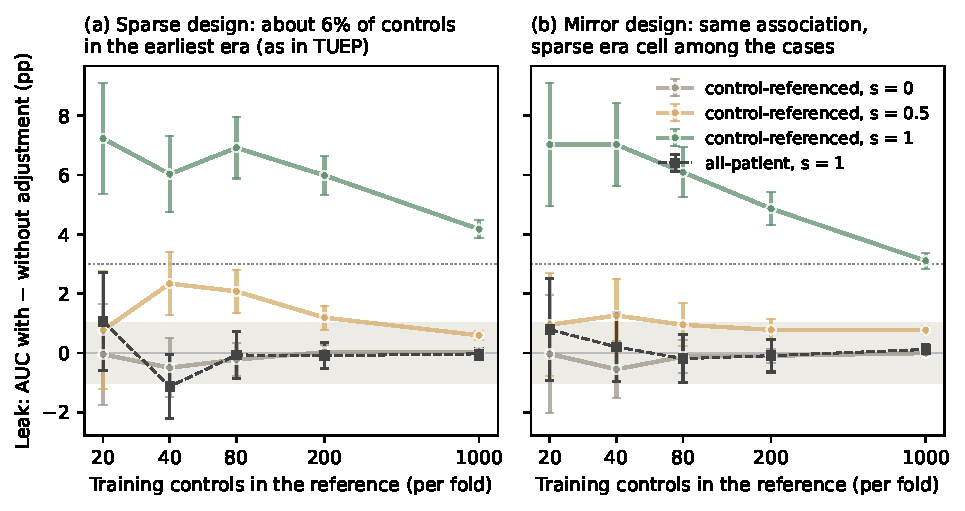
\includegraphics[width=\textwidth]{Fig4.pdf}
\caption{Leak of the control-referenced adjustment in the control-reference simulation (patient-level logistic regression, 100 replicates per point): mean paired difference in pooled AUC with Monte Carlo 95\% CIs by number of reference controls and label--covariate association $s$. (a) Sparse design, as in TUEP. (b) Mirror design, sparse era cell among the cases. Dashed, all-patient adjustment at $s=1$; shading and dotted line, paired-rule mean thresholds. AUC, area under the receiver operating characteristic curve, in percentage points (pp); CI, confidence interval; TUEP, Temple University Hospital EEG Epilepsy Corpus.}\label{fig:referensi}
\end{figure}

\subsection{Properties of the audit rules}\label{sec:oc}

The next question was how often the two rules misjudge such leaks (\tabref{tab:oc}).

In the independent audits, the rules declared leakage in 0 of 48 null audits (Clopper--Pearson 95\% CI 0.0\%--7.4\%). The combined decision detected all 48 leaking audits (95\% CI 92.6\%--100\%), and the absolute rule alone detected 33. Near-margin cells (means of 1.7--2.4 pp over the new replicates) gave ``uncertain'' in 32 of 40 audits of 20 and ``leakage'' in 4. Audits of 50 or 100 replicates gave ``leakage'' in 0 of 24 (S2.18).

\begin{table}[!htb]
\caption{Decisions of the audit rules by scenario, audit size $n$, and rule: all leaking simulation audits were detected.}\label{tab:oc}
\centering\scriptsize
\setlength{\tabcolsep}{2.5pt}
\begin{adjustbox}{max width=\textwidth}
\begin{tabular}{p{0.33\textwidth}ccccc}
\toprule
Scenario & $n$ (audits) & R1 & R2 & Combined \\
\midrule
\multicolumn{5}{l}{\textit{(a) Independent audits of new simulation replicates (counts of audits)}} \\
Null cells (3) & 20 (30) & 29/1/0 & 27/3/0 & 26/4/0 \\
 & 50 (12) & 12/0/0 & 12/0/0 & 12/0/0 \\
 & 100 (6) & 6/0/0 & 6/0/0 & 6/0/0 \\
Near-margin cells (4) & 20 (40) & 21/19/0 & 5/31/4 & 4/32/4 \\
 & 50 (16) & 11/5/0 & 1/15/0 & 1/15/0 \\
 & 100 (8) & 6/2/0 & 0/8/0 & 0/8/0 \\
Leaking cells (3) & 20 (30) & 0/10/20 & 0/0/30 & 0/0/30 \\
 & 50 (12) & 0/3/9 & 0/0/12 & 0/0/12 \\
 & 100 (6) & 0/2/4 & 0/0/6 & 0/0/6 \\
\midrule
\multicolumn{5}{l}{\textit{(b) Draws from stored pools (percent of draws, mean over pools [maximum leakage])}} \\
Plasmode $\gamma=0$, null (18 pools) & 20 & 94.8/5.2/0.0 & 70.3/26.6/3.1 & 68.9/28.0/3.1 [14.6] \\
 & 50 & 99.5/0.5/0.0 & 77.2/21.5/1.4 & 77.2/21.5/1.4 [4.4] \\
 & 100 & 100.0/0.0/0.0 & 79.2/20.6/0.2 & 79.2/20.6/0.2 [0.9] \\
Simulation, null (41 cells) & 20 & 96.0/4.0/0.0 & 90.7/8.9/0.3 & 87.3/12.4/0.3 [8.1] \\
 & 50 & 98.6/1.4/0.0 & 98.5/1.5/0.0 & 97.1/2.9/0.0 [0.1] \\
Plasmode $\gamma=1$, leaking (5 pools) & 20 & 0.0/0.0/100.0 & 0.0/0.0/100.0 & 0.0/0.0/100.0 \\
Simulation, leaking (55 cells) & 20 & 2.3/15.5/82.2 & 0.0/3.8/96.2 & 0.0/3.5/96.5 \\
V0, strict nesting (100) & 20 & 0.1/50.2/49.8 & 0.0/0.8/99.2 & 0.0/0.5/99.5 \\
 & 100 & 0.0/51.5/48.5 & 0.0/0.0/100.0 & 0.0/0.0/100.0 \\
\bottomrule
\end{tabular}
\end{adjustbox}

\vspace{2pt}
\begin{minipage}{\textwidth}\footnotesize
Entries, no evidence/uncertain/leakage. (a) Independent audits of new simulation replicates, non-overlapping within each $n$ and shared across sizes (per cell, S2.18). (b) Bootstrap draws from stored pools of 20--120 replicates (pool-resampling confidence intervals, S2.17). R1, absolute rule; R2, paired rule; combined, leakage if either rule declares it and no evidence only if both do; V0, control-referenced adjustment.
\end{minipage}
\end{table}%

In pool draws on recorded features without a label--covariate association (plasmode $\gamma=0$), the combined decision inherited the false alarms of the paired rule: 3.1\% of draws of 20 on average and up to 14.6\% in one of 18 pools. Audits of 50 and 100 replicates gave fewer false alarms (\tabref{tab:oc}). A likely reason is that raw tree pools of 120 replicates had positive residual means of +0.9 to +1.1 pp with SDs of 7.5 to 8.0 pp (S2.11). With strict nesting, the control-referenced pipeline sat at the absolute threshold (pooled AUC 55.0), and the absolute rule detected it in 49.8\% of draws of 20, the combined decision in 99.5\% (S2.19).

The number of replicates planned with \eqref{eq:n} is sensitive to the pilot mean. A raw random forest at $\gamma=0$ illustrates the sensitivity: the 120-replicate pool ($b=1.1$, $\hat{\sigma}_{\Delta}=8.0$ pp) requires 95 replicates, and its one-sided 80\% upper bound of $b$ (1.7 pp) requires 205. The first 20 replicates of that pool, used as a pilot ($b=2.9$ pp), require 16,664, and the upper bound of that pilot mean exceeds 3 pp, where \eqref{eq:n} has no solution (S2.19).

\subsection{The audited pipeline on the clinical label}\label{sec:kinerja}

Finally, the audit was applied to a clinical-label performance figure. With all-patient adjustment, the fusion pipeline reached a per-fold AUC of 69.7 on the clinical label, and its advantage over an acquisition-metadata baseline (65.5) was not significant ($p = 0.45$, Nadeau--Bengio corrected $t$-test \cite{nadeau2003}). The undetected benefit of EEG does not establish equivalence (S3.5).%
\section{Discussion}\label{sec:discussion}

\subsection{Main findings and mechanisms}\label{sec:disk_temuan}

Covariate adjustment made uninformative EEG features look informative only for some combinations of classifier, fitting level, feature distribution, and reference sample. Least-squares adjustment fitted on units $\mathcal{F}$ with weights $w_j$ yields residuals satisfying $\sum_{j\in\mathcal{F}} w_j\mathbf{z}_j\mathbf{d}_j^{\top}=\mathbf{0}$. A linear classifier trained on units $\mathcal{T}$ with weights $v_j$, however, sees the covariates through $\sum_{j\in\mathcal{T}} v_j\mathbf{z}_j\mathbf{d}_j^{\top}$, which differs from zero unless $\mathcal{T}=\mathcal{F}$ and $v=w$. The property is orthogonality on the fitting units, not independence from covariates or label, and leaves the test AUC free to depart from 50. Orthogonality also requires equal weights, which balanced class weights provide only for balanced training classes (80 per class in the TUEP folds, unlike Emotiv), and median-based features computed after mean-based adjustment break it. Leakage appeared where the condition was broken, although the leaking configurations also differed in tails, sample sizes, weights, and pooling. Matching the training configuration of window-level logistic regression to the adjustment removed about 60\% of the TUEP leak. The remaining +2.8 pp (95\% CI +1.5 to +4.0, ``uncertain'') describes this TUEP configuration, whereas all Emotiv variants stayed at or below +1.2 pp. Attribution to the fitting unit is withheld, because the patient-level comparison also differed in feature summary and aggregation.

In nonlinear classifiers, covariate information can persist in the spread and tails of heavy-tailed features \cite{hamdan2023}. Because the Bi-LSTM still leaked +4.1 pp after rank-normal, the leak does not reside in the marginal tails alone. A transformation modifies the regression rather than replacing it, as stratification would \cite{hamdan2023}; hence, the feature-shuffle test remains necessary after a transformation.

Control-referenced adjustment broke the condition through its reference sample. In one training fold, the largest residual-on-design coefficient was $3.9\times10^{-15}$ for the training controls, against 1.39 for the training patients with epilepsy (S2.9). A plausible explanation is that coefficient error adds a linear function of the covariates to the features of each patient outside the reference, which a classifier can exploit because the label is associated with the covariates. Consistent with this explanation, the simulated leak vanished without a label--covariate association and shrank as the reference grew. The half-reference variant, whose reference controls were excluded from classifier training, leaked as well. A random reference holding both classes leaked less (+1.7 against +4.3 pp with strict nesting). When the reference excludes one class, the injected shift separates the classes during training.

The two rules complement each other: the absolute rule missed 10 of 30 leaking audits of 20 replicates and half of the draws of the nested control-referenced pipeline, because it judges the adjusted AUC rather than its change. Being more sensitive, the paired rule had false alarms that depended on the pool and reached 14.6\% on null plasmode data. Combined, the rules detected all 48 leaking simulation audits, whereas near-margin leaks stayed ``uncertain'' and call for more replicates.

\subsection{Implications for audits of clinical data}\label{sec:implikasi}

Besides splitting by patient \cite{delpup2025,brookshire2024,rosenblatt2024}, developers and archive managers can apply four provisional checks before reading archive performance as disease information.
\begin{itemize}[leftmargin=*,itemsep=0pt,topsep=2pt]
\item (1) Run the feature-shuffle test with and without adjustment for nonlinear and window-level classifiers, even after a transformation \cite{hamdan2023}, and judge the result with both rules combined, as a complement to the partial confounder test \cite{spisak2022}.
\item (2) Test likewise any adjustment whose reference differs from the training patients of the classifier, as in normative-style adjustment \cite{rutherford2022,kia2022}, because a reference of 1,000 controls per fold still leaked in simulation.
\item (3) Plan the replicates with \eqref{eq:n} from a pilot of the same pipeline on a negative control, using an upper bound of the pilot mean $b$. A pilot mean near 3 pp inflates $n$ without bound, and \tabref{tab:oc} gives the frequencies of the combined decision.
\item (4) Report an acquisition-metadata baseline beside each performance figure.
\end{itemize}

\subsection{Limitations}\label{sec:batasan}

Recorded EEG features came from one retrospective archive of 200 patients and one public cohort, and the results concern auditing rather than clinical use. The two rules use conventional thresholds and were checked on ten simulation cells, with the control-referenced adjustment and its variants as the positive controls on recorded features. Replication in the Emotiv cohort covered the nonlinear plasmode leak, whereas the reference experiments used TUEP alone, one linear classifier, and normal simulated features. The audited adjustments were ordinary least-squares regressions with homoscedastic scaling, simpler than warped normative models \cite{fraza2021}, and each leak rests on one hyperparameter configuration and artifact threshold \cite{kessler2025}. Strict nesting was repeated only for the control, random, and all-patient references, and S4.3 lists further limitations.%
\section{Conclusion}\label{sec:conclusion}
Covariate adjustment can manufacture discrimination from electroencephalography (EEG) without label information, depending in these data on its fitting population and training configuration. (i) Adjusting raw EEG features added about 11 percentage points (pp) of discrimination to nonlinear classifiers in two cohorts. In the clinical archive, window-level logistic regression with the tree training configuration gained 6.6 pp (2.8 pp with a matched configuration), against at most 1.1 pp on patient-level features. (ii) Fitted only on the training controls, the adjustment leaked into a linear patient-level classifier with strict nesting, more than a random reference of equal size in this cohort composition. (iii) The frozen rules raised 0 false alarms in 48 leakage-free simulation audits and detected all 48 leaking ones, whereas semi-synthetic data without a label--covariate association gave false alarms in up to 14.6\% of draws of 20. A pilot-based rule sets the number of shuffles that keeps paired-rule false alarms below 1\% under a normal model when the pilot mean stays well below 3 pp.

A performance figure from stored clinical EEG after covariate adjustment should therefore be reported with a feature-shuffle test run with and without adjustment, a replicate number planned from a pilot, and an acquisition-metadata baseline. The audit needs only features, labels, and covariates, so it can be run on other patient-clustered clinical data, where its rule error frequencies are measured in the same way.%
\section*{CRediT authorship contribution statement}
\textbf{Miftah Furqaanul Haq:} Conceptualization, Methodology, Software, Investigation, Writing -- original draft. \textbf{Dwi Sunaryono:} Supervision, Resources, Writing -- review \& editing. \textbf{Muhammad Hasan Basri:} Data curation, Formal analysis, Writing -- review \& editing.

\section*{Declaration of competing interest}
The authors declare that they have no known competing financial interests or personal relationships that could have appeared to influence the work reported in this paper.

\section*{Funding}
This research did not receive any specific grant from funding agencies in the public, commercial, or not-for-profit sectors.

\section*{Data availability}
\begingroup\emergencystretch=2em\Urlmuskip=0mu\relax TUEP v2.0.1 is distributed by the Neural Engineering Data Consortium to registered users under its data use terms \cite{obeid2016,veloso2017}, which reserve redistribution to the consortium. The Emotiv cohort is a public release on Zenodo (1252141) \cite{vanhees2018}. The code, software environment, fold assignments, seeds, analysis plans, and table scripts are available at \url{https://github.com/miftahfurqaanul/Auditing-covariate-adjustment-leakage-in-patient-level-EEG-TUEP}. S2.20 maps each main-text table and figure to its script (with SHA-256 prefix), seeds, and output files.\par\endgroup

\section*{Declaration of generative AI and AI-assisted technologies in the manuscript preparation process}
During the preparation of this work the authors used Claude (Anthropic) to improve the language and readability of the manuscript and to draft the graphical abstract. After using this tool, the authors reviewed and edited the content as needed and take full responsibility for the content of the published article.%   %

\bibliographystyle{elsarticle-num}
\bibliography{referensi}

\end{document}

\endinput
